% !TeX root = ../report.tex

\section{Deep Learning}
In this section we will go through an overview of the model used in the "deep learning" attempt at solving the task at hand. The model seeks to solve to sub task in one go, namely: regression (task 1 in section 1.1) and classification (task 5 in section 1.1). For task one the model also predicts independently of the general emotion felt, i.e. tweets for joy, anger etc. get a 0-to-1 score using the same model.

\subsection{Model overview}

\subsubsection{Preprocessing of text and textual representation} \label{sec:preprop}
For the textual preprocessing, all tweets are read in and converted using a mapping from the word to an integer. This ensures that words get mapped to the same key and also enables an enforcing on the maximal amount of words to be used. Train data is treated differently than development and test data, in that every word read in train data gets converted to a word vectors independently based on the word but if an unknown word gets read in the development or test data its numerical value gets replaced by an "unknown" placeholder. One way of countering this is to use pretrained word embeddings. This does not constitute as having read and adapted to the test set, since one could envision having a pretrained word embedding for every word in the entire language.

\subsubsection*{Augmentation of data}
MODIFICER HVIS VI LAVER NOGET ANDET.\\
The first iteration of the data augmentation consisted of reading in all the data for task 1 and 5 as described in section \ref{sec:preprop}. Since the tweets had different format of truth labels, one was a singular value (regression) and one was a multilabel list (classification), reading in the labels had to be augmented. When reading in a regression tweet the model would augment by append 11 dimensions extra for the binary flag values and when reading in a classification tweet the model prepend one extra dimension. All these augmented truth labels would be instantiated to -1, and this value would then act as a flag for later usage in loss function calculation.

\subsubsection{Model architecture}
\begin{figure}[H]
    \centering
    \begin{subfigure}[b]{0.3\textwidth}
        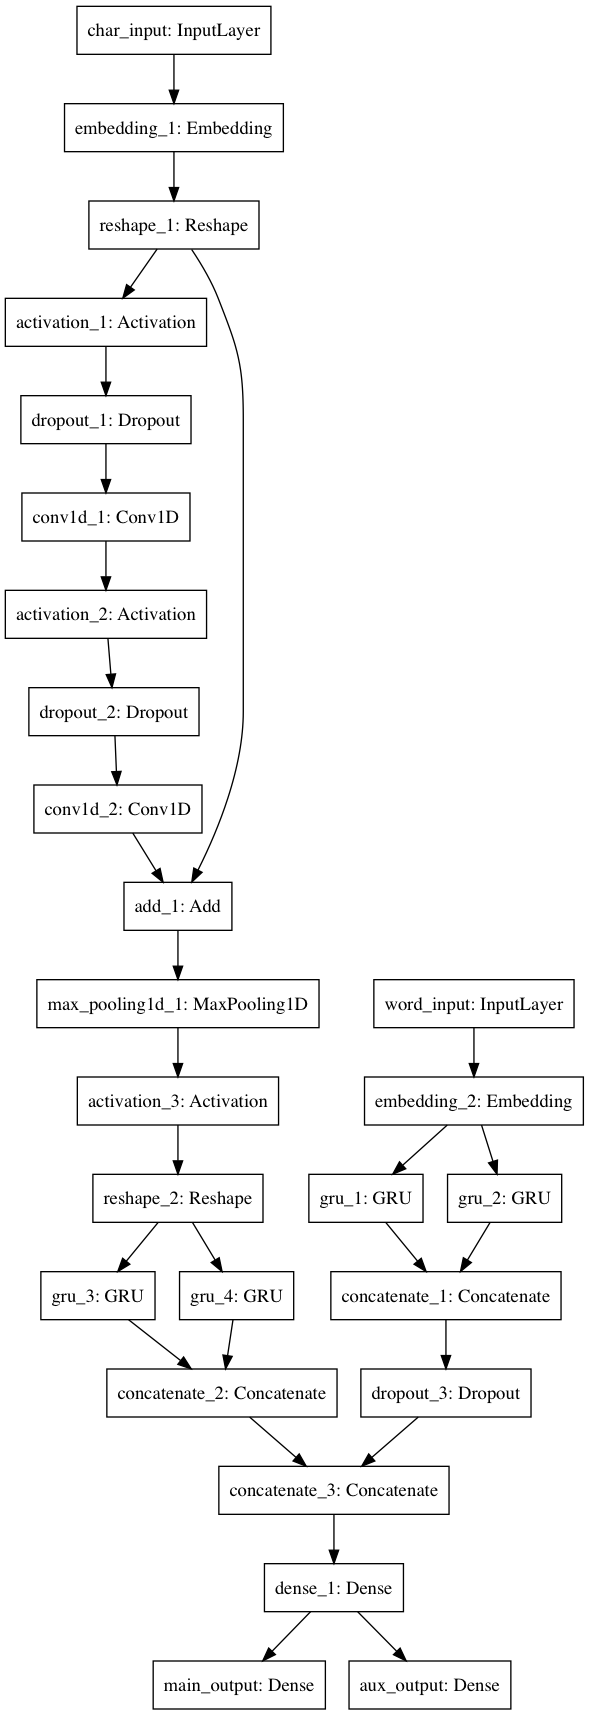
\includegraphics[width=\textwidth]{pictures/model_full.png}
        \caption{The full model}
        \label{fig:model_full}
    \end{subfigure}
    \begin{subfigure}[b]{0.3\textwidth}
        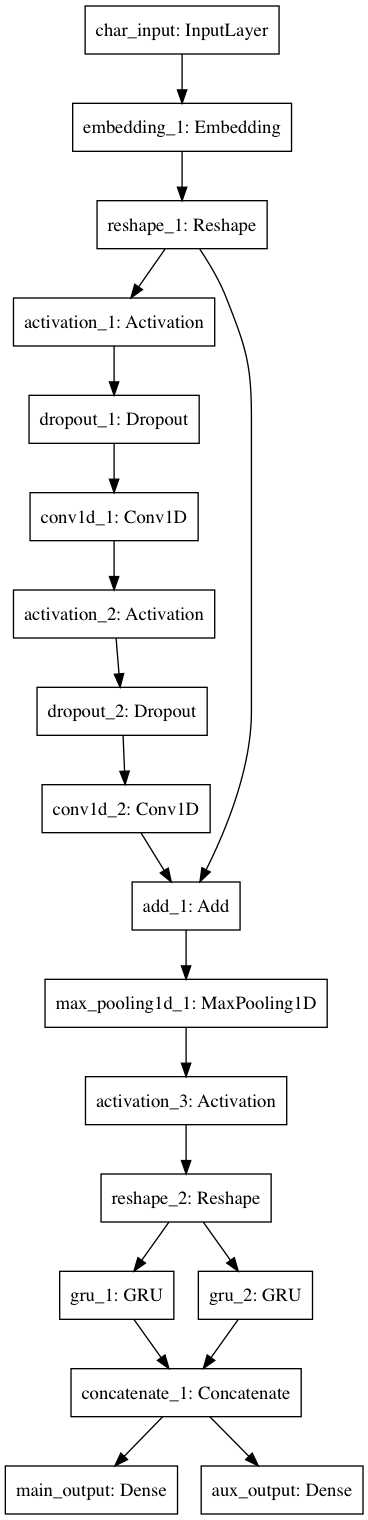
\includegraphics[width=\textwidth]{pictures/model_chars.png}
        \caption{The model only training on char representations}
        \label{fig:model_chars}    
    \end{subfigure}
    \begin{subfigure}[b]{0.3\textwidth}
        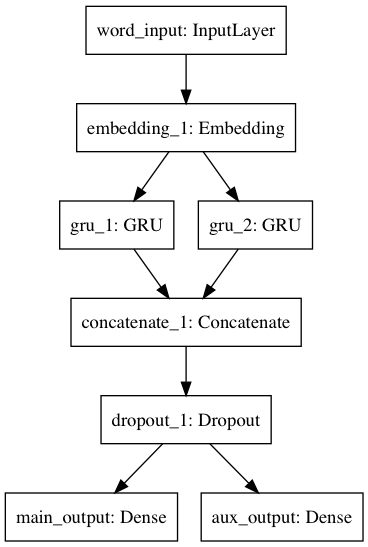
\includegraphics[width=\textwidth]{pictures/model_words.png}
        \caption{The model only training on word representations}
        \label{fig:model_words}
    \end{subfigure}
\end{figure}
